% Created 2016-05-02 Mon 15:15
\documentclass[11pt]{article}
\usepackage[utf8]{inputenc}
\usepackage{lmodern}
\usepackage[T1]{fontenc}
\usepackage{fixltx2e}
\usepackage{graphicx}
\usepackage{longtable}
\usepackage{float}
\usepackage{wrapfig}
\usepackage{rotating}
\usepackage[normalem]{ulem}
\usepackage{amsmath}
\usepackage{textcomp}
\usepackage{marvosym}
\usepackage{wasysym}
\usepackage{amssymb}
\usepackage{amsmath}
\usepackage[version=3]{mhchem}
\usepackage[numbers,super,sort&compress]{natbib}
\usepackage{natmove}
\usepackage{url}
\usepackage{minted}
\usepackage{underscore}
\usepackage[linktocpage,pdfstartview=FitH,colorlinks,
linkcolor=blue,anchorcolor=blue,
citecolor=blue,filecolor=blue,menucolor=blue,urlcolor=blue]{hyperref}
\usepackage{attachfile}
\usepackage[left=1in, right=1in, top=1in, bottom=1in, nohead]{geometry}
\geometry{margin=1.0in}
\usepackage{amsmath}
\usepackage{graphicx}
\usepackage{epstopdf}
\usepackage{fancyhdr}
\usepackage{hyperref}
\usepackage[labelfont=bf]{caption}
\usepackage{setspace}
\setlength{\headheight}{10.2pt}
\setlength{\headsep}{20pt}
\def\dbar{{\mathchar'26\mkern-12mu d}}
\pagestyle{fancy}
\fancyhf{}
\renewcommand{\headrulewidth}{0.5pt}
\renewcommand{\footrulewidth}{0.5pt}
\lfoot{\today}
\cfoot{\copyright\ 2016 W.\ F.\ Schneider}
\rfoot{\thepage}
\chead{\bf{Introduction to Chemical Engineering (CBE 20255)\vspace{12pt}}}
\lhead{\bf{Homework 10}}
\rhead{\bf{Due April 29, 2016}}
\usepackage{titlesec}
\titlespacing*{\section}
{0pt}{0.6\baselineskip}{0.2\baselineskip}
\title{University of Notre Dame\\Introduction to Chemical Engineering\\(CBE 20255)}
\author{Prof. William F.\ Schneider}
\def\dbar{{\mathchar'26\mkern-12mu d}}
\usepackage{siunitx}
\setcounter{secnumdepth}{3}
\author{William F. Schneider}
\date{\today}
\title{CBE 60553 Outline}
\begin{document}

\begin{options}
\end{options}

\noindent \textbf{Solve each problem on a separate sheets of Engineering Computation paper.  Carefully and neatly document your answers. Box your final answer, reporting it with the correct number of significant figures and units.  Use plotting software for all plots.}


\section{Hot acid in a closed container}
\label{sec-1}
You are going to dilute 2.00 mol of 100\% \ce{H2SO4} with enough water to make a 30\%(mol/mol) solution.  Both acid and \ce{H2O} are initially at \SI{25}{\celsius}. Table B.11 is a convenient source of enthalpy of mixing data, and Perry's reports the specific heat of aqueous \ce{H2SO4} to be:

\begin{center}
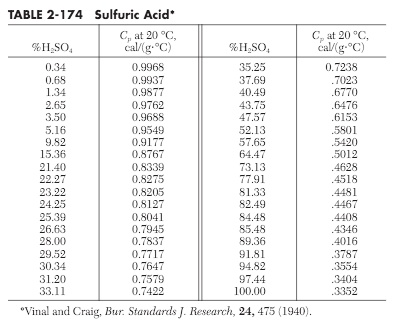
\includegraphics[width=0.5\textwidth]{../../figs/H2SO4-Cp.png}
\end{center}

\begin{enumerate}
\item (4 pts) How much cooling (kJ) is necessary to maintain the final solution at \SI{25}{\celsius}?
\item (4 pts) Suppose you do this mixing in a well-insulated \SI{150}{\gram} flask that has a heat capacity of \SI{3.30}{\joule\per\gram\per\celsius}.  What is the final temperature of the solution?
\item (4 pts) In a separate experiment, you have an \ce{H2SO4} solution of unknown compositionBelow is an enthalpy-concentration chart for \ce{H2O}/\ce{H2SO4}.  Draw an appropriate line on it to estimate the final temperature if the mixing is done adiabatically.
\end{enumerate}

\begin{center}
\includegraphics[width=0.45\textwidth]{../../figs/H2SO4-Enthalpy.png}
\end{center}


\section{Trying to concentrate}
\label{sec-2}
A 0.1\%(mol/mol) caustic soda (NaOH) solution is to concentrated in a continuous evaporator. The solution enters the evaporator at \SI{25}{\celsius} at a rate of \SI{150}{\mole\per\minute} and exits at 5\%(mol/mol) and \SI{60}{\celsius}.  Hot dry air is bubbled into the evaporator at \SI{200}{\celsius} and 1.1 bar absolute and leaves as saturated air at \SI{60}{\celsius} and 1 atm. Because the liquid solutions are fairly dilute, you can assume their heat capacities to be the same as that of pure \ce{H2O}.

\begin{enumerate}
\item (4 pts) Sketch a process diagram for this unit operation, labeling all inputs and outputs.
\item (2 pts) What is the composition of the exiting saturated air?
\item (4 pts) What are the molar flow rates of all streams? (Recall that dry air can be treated as a single compound with an effective MW).
\item (4 pts) What is the volumetric flow rate of dry air?
\item (8 pts) Create an enthalpy table (kJ/mol) for all inlet and exit species.  Take as your enthalpy references the inlet caustic acid solution, dry air at \SI{25}{\celsius}, and \ce{H2O} at \SI{25}{\celsius}. Identify the tables from the text you use for each calculation.
\item (4 pts) Use an enthalpy balance to determine the required heat or cooling to maintain the target temperature.
\end{enumerate}


\section{Get oily clean}
\label{sec-3}
Trichloroethylene (TCE) is a common industrial cleaning solvent, produced by chlorinating ethylene:

\[\ce{C2H4 (g) + 2 Cl2 (g) -> C2H2Cl4 (l) + H2 (g)},\quad \Delta \hat{H}^{\circ}_{r} = \SI{-385.76}{\kilo\joule\per\mole} \]

\noindent followed by dehydrochlorination of tetrachloroethane:

\[ \ce{C2H2Cl4 (l) -> C2HCl3 (l) + HCl (g)}\]

\noindent The standard heat of formation of TCE, \(\Delta H^{\circ}_\text{f,TCE} = \SI{-276.2}{\kilo\joule\per\mole} \), and other necessary standard heats are in Table B.1 of the text.

\begin{enumerate}
\item (2 pts) What is the standard heat of formation of \ce{C2H2Cl4 (l)}?
\item (2 pts) What is the standard heat of the second reaction?
\item (2 pts) What is the standard enthalpy of the net reaction for making TCE from ethylene and \ce{Cl2}?
\item (2 pts) Suppose a process generates 300 mol/hr of TCE, with all reactants and products at 1 atm and \SI{25}{\celsius}.  How much heat must be added to or removed from the process?
\end{enumerate}
\section{A shifty reaction}
\label{sec-4}
Water-gas shift (WGS) is an important industrial reaction for generating \ce{H2} from carbon monoxide:

\[ \ce{ CO(g) + H2O (g) -> CO2 (g) + H2 (g) }\]

\noindent CO at \SI{25}{\celsius} and steam at \SI{150}{\celsius} are fed to a WGS reactor.  The effluent contains 40.0\% \ce{H2}, 40.0\% \ce{CO2}, and balance steam at \SI{500}{\celsius} and a flow rate of 3.50 standard cubic meters per hour.  This effluent passes to a condenser to drop out the \ce{H2O}.  Gas and liquid streams leave the condenser at 1 atm and \SI{15}{\celsius}.  The Henry's Law constants of \ce{H2} and \ce{CO2} are large enough to neglect their solubility in the liquid water.

\begin{enumerate}
\item (4 pts) Sketch and label the overall process.
\item (4 pts) Compute the inlet molar flow rates of CO and steam.  If either is in excess, explain why the process is designed in such a way.
\item (4 pts) Compute the molar flow rate of exiting liquid water and of the vapor phase.
\item (4 pts) Do an enthalpy balance on the condenser and determine the rate at which it must be heated or cooled (kW).
\item (2 pts) What is the standard enthalpy of WGS?
\item (2 pts) What is the reaction advancement in the reactor?
\item (4 pts) Create an enthalpy table for the reactor based on the ``heat of formation'' method.
\item (4 pts) Do an enthalpy balance on the reactor and determine the rate at which it must be heated or cooled (kW).
\item (4 pts) It has been suggested that the inlet CO and reactor effluent could be passed through opposite sides of a heat exchanger before the effluent is sent to the condenser. Sketch such a process and explain why this might make sense. (This concept is called ``heat integration.'')
\end{enumerate}

\section{\textbf{BONUS} \textbf{BONUS} \textbf{BONUS}}
\label{sec-5}
(For those of you looking for some extra points or an extra challenge.)  Ammonia is oxidized to make nitric oxide in a well-insulated flow reactor:

\[\ce{4 NH3(g) + 5 O2(g) -> 4 NO(g) + 6 H2O(g)},\quad \Delta H^{\circ}_{r}=\SI{-904.7}{\kilo\joule\per\mole}\]

\noindent The feed stream enters at \SI{200}{\celsius} with 4.00 and \SI{6.00}{\mole\per\second} \ce{NH3} and \ce{O2}, respectively.  The \ce{NH3} conversion in 100\%, and the products exit at some unknown temperature \emph{T}.

\begin{enumerate}
\item (4 pts) Sketch and label a process flow chart for this process.
\item (6 pts) Perform a mass balance to determine the flow rates of all products and the reaction extent.
\item (2 pts) Now you need to perform an enthalpy balance.  Which method do you choose, heat of reaction or heat of formation?
\item (4 pts) Compute the specific enthalpies of the reactants based on your choice.
\item (6 pts) Write expression for the specific enthalpies of the products based on your choice.  Take advantage of the heat capacities in Table B.2.
\item (6 pts) Based on your enthalpy balance, what is the temperature of the exiting gases?  This requires you to solve a non-linear equation.  State the method you use and show intermediate results.
\item (4 pts) I'm pretty lazy at heart.  Suppose I solved this problem using only the leading, constant terms for the heat capacities of the products.  The problem is then much easier to solve.  What temperature would I get, and how far off am I?  Does it pay to be lazy?
\end{enumerate}
% Emacs 25.0.50.1 (Org mode 8.2.10)
\end{document}